\documentclass[12pt]{article}

\usepackage{graphicx}
\usepackage{float}
\usepackage{subcaption}
\usepackage{amsfonts}
\usepackage{amsmath}
\usepackage{amssymb}
\usepackage[margin=1in, paperheight=11in, paperwidth=8.5in]{geometry}

\title{Progress Report: Parallel Controllable Texture Synthesis}
\author{Matthew McMullan and Ian Ooi}
\date{December 4, 2012}

\begin{document}
    \maketitle
    \section{Current Progress}
        So far, we have implemented upsampling and jitter, the first two steps of the general algorithm.  Our upsampling implementation uses a fragment shader which renders a series of textures to produce an image pyramid.  The fragment shader produces the different sizes of images by starting at a 1 pixel by 1 pixel texture of coordinates (where the coordinates correspond to coordinates in the exemplar).  Every round, the number of pixels quadruples, with each pixel creating an extra pixel to the right, below it, and diagonally to the right and below.  The pixels of the image are shifted to accommodate the extra pixels, and the new pixels are filled with the pixel coordinates from the exemplar.
        
      Jitter is accomplished through the use of a simplex noise implementation. We modify the destination locations in each level of the image pyramid with deterministically calculated pseudo-random noise, with each pixel of the result storing the pixel coordinates of a texel in the exemplar.  We choose a direction to shift the pixel, either $+1$ or $-1$ based on a randomness threshold ratio $r$ individually for the x and y directions.  In order to have higher values of $r$ correspond to more randomness, the comparison is made between the generated noise value $\vec{n} \in \mathbb{R}^2$ and the quantity $\left(1 - r \right)$, where $n_i > (1-r)$ corresponds to a $+1$ and $n_i < -(1-r)$ corresponds to $-1$, with any other value resulting in no movement (a $0$).  The position of the pixel-coordinate texel is then moved accordingly.  Throughout upsampling and jitter, we only work with pixel coordinates, not the actual values of the exemplar.
        
        \subsection{Implementation}
            There have been a few changes in the method in which we're implementing this algorithm.  Due to some limitations of the Unity 3D Engine, we have moved to using OpenGL with GLFW for our implementation.  Instead of Cg shaders, we are now utilizing GLSL shaders, and the visualizations of our results are done by rendering the texture on a single quad.  The rendering takes place in a rendering context within the GLFW window, which also handles our key callbacks for operations such as switching between which level of the pyramid is displayed and for re-loading the shaders.

    \section{Preliminary Results}
        \begin{figure}[H]
            \centering
            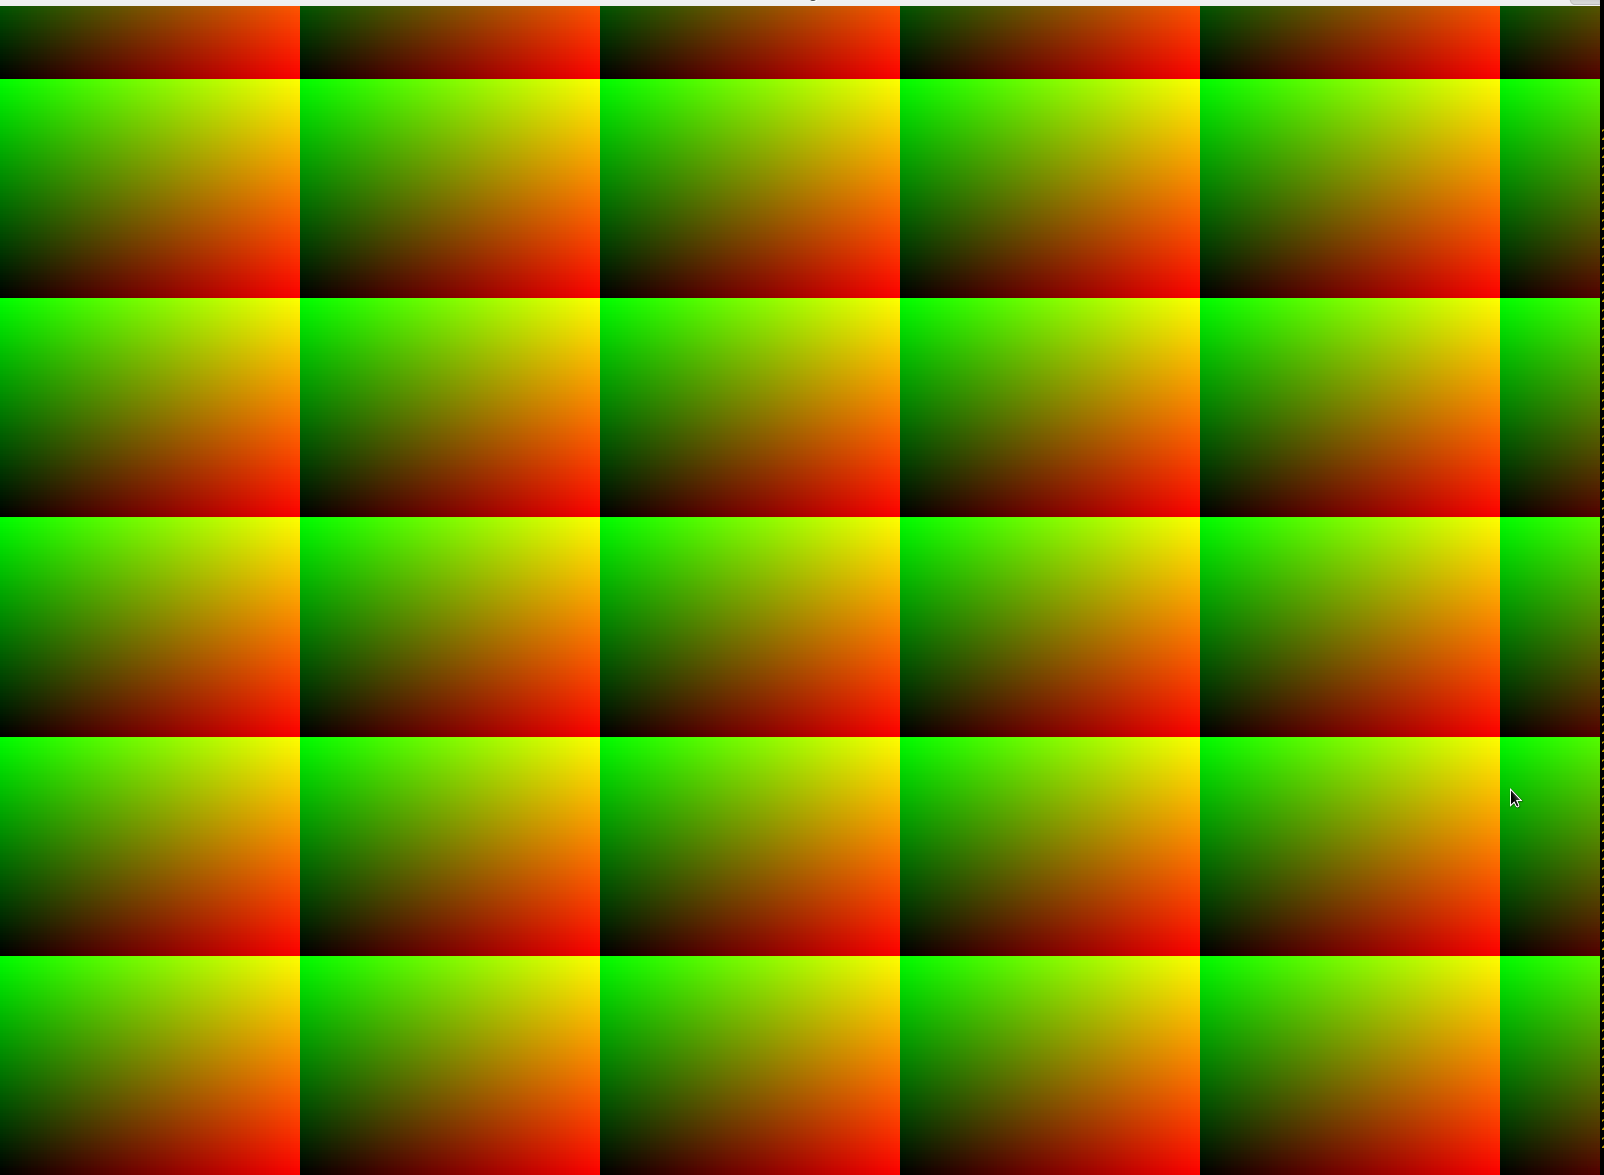
\includegraphics[width=2.5in]{result3.png}
            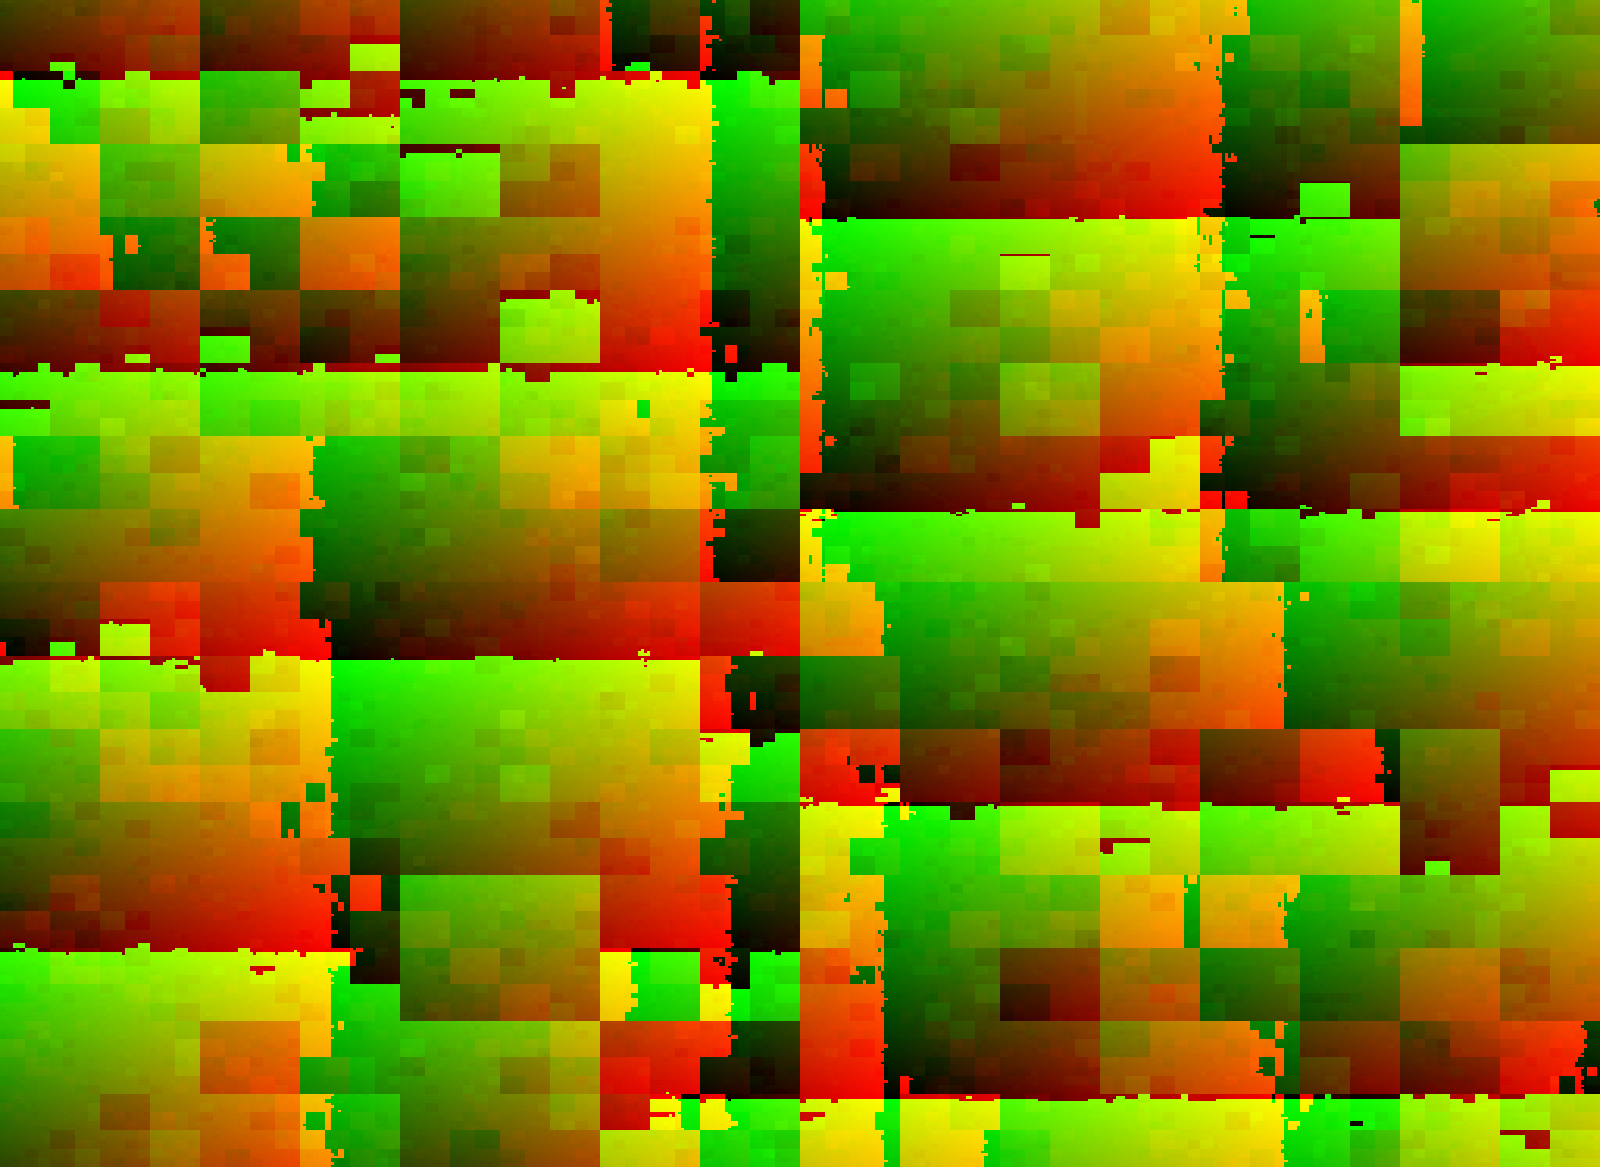
\includegraphics[width=2.5in]{result0.png}
            \caption{We show a visualization of our upscaling and jitter on a gradient (right), as pictured in the leftmost image above.}
        \end{figure}
        \begin{figure}[H]
            \centering
            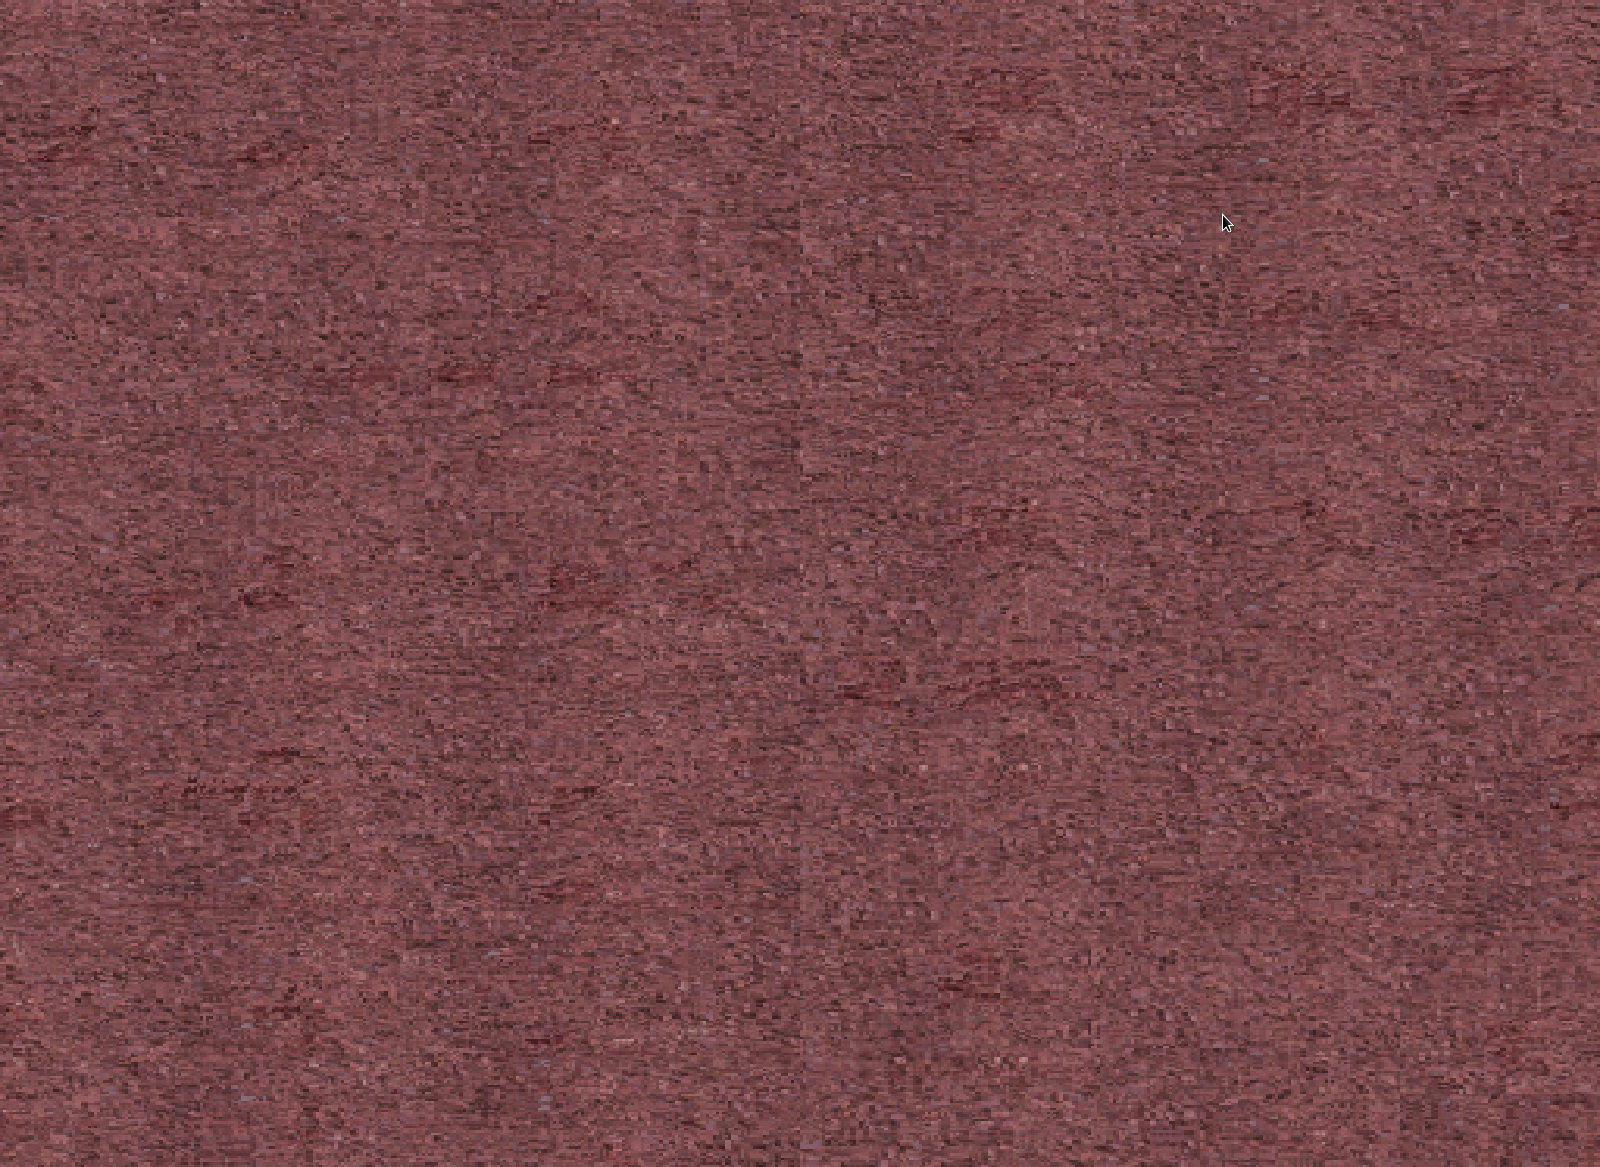
\includegraphics[width=2.5in]{result1.png}
            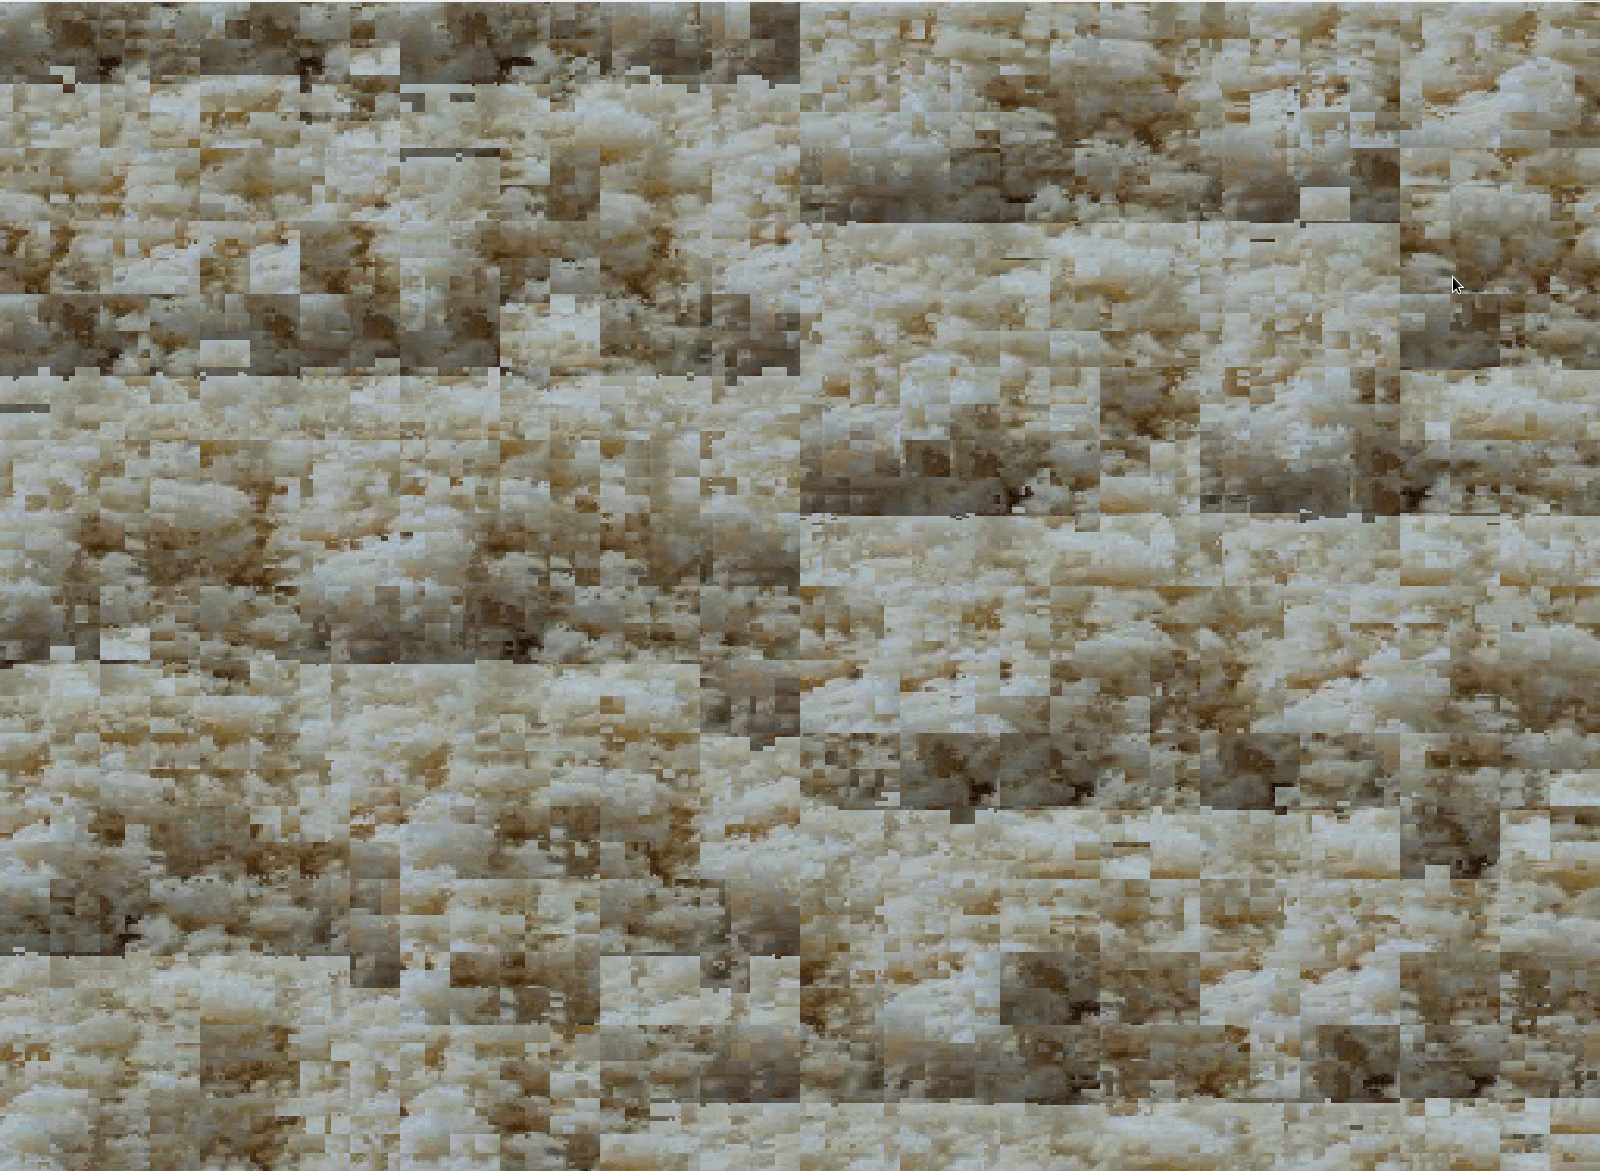
\includegraphics[width=2.5in]{result2.png}
            \caption{Two samples of upscaled and jittered textures at the highest scale in the pyramid.}
        \end{figure}
\end{document}
